\begin{figure}[H]
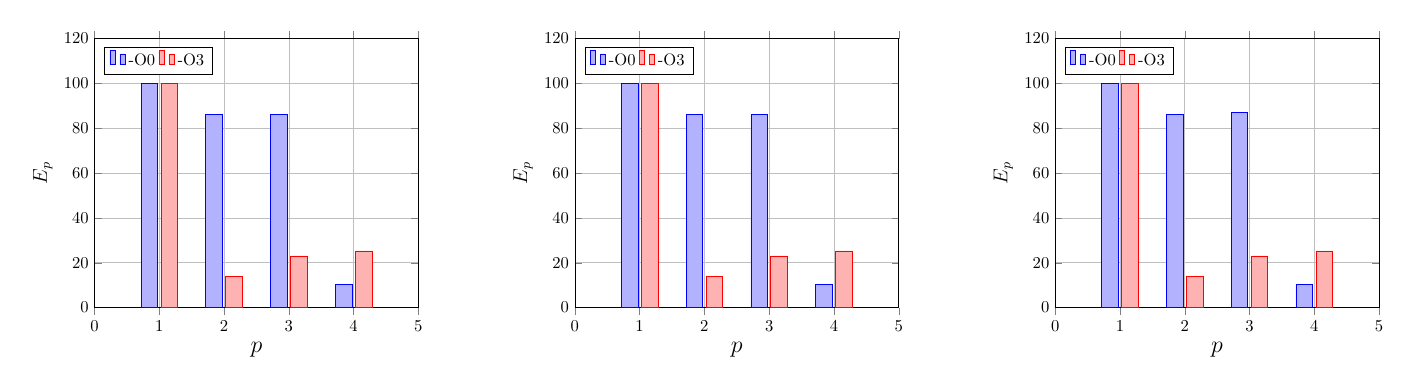
\begin{tikzpicture}
\begin{scope}[scale=0.6]
\begin{axis}[
 ybar,
 xmin=0, ymin=0,
 ymax=120,  xmax=5, %32
 xlabel={\Large $p$}, ylabel={\large $E_p$},
 grid=major,
legend columns=-1,
legend pos= north west,
tick=empty
]
\addplot coordinates {(1,100) (2, 86.3) (3, 86) (4, 10.2)};
\addlegendentry{-O0}
\addplot coordinates {(1,100) (2, 14.) (3, 23.) (4, 25.3)};
\addlegendentry{-O3}
\end{axis}
\end{scope}
\begin{scope}[xshift=6.1cm,scale=0.6]
\begin{axis}[
 ybar,
 xmin=0, ymin=0,
 ymax=120,  xmax=5, %32
 xlabel={\Large $p$}, ylabel={\large $E_p$},
 grid=major,
legend columns=-1,
legend pos= north west,
tick=empty
]
\addplot coordinates {(1,100) (2, 86.) (3, 86.) (4, 10.2)};
\addlegendentry{-O0}
\addplot coordinates {(1,100) (2, 14.) (3, 23.) (4, 25.3)};
\addlegendentry{-O3}
\end{axis}
\end{scope}
\begin{scope}[xshift=12.2cm,scale=0.6]
\begin{axis}[
 ybar,
 xmin=0, ymin=0,
 ymax=120,  xmax=5, %32
 xlabel={\Large $p$}, ylabel={\large $E_p$},
 grid=major,
legend columns=-1,
legend pos= north west,
tick=empty
]
\addplot coordinates {(1,100) (2, 86.3) (3, 86.9) (4, 10.2)};
\addlegendentry{-O0}
\addplot coordinates {(1,100) (2, 14.) (3, 23.) (4, 25.3)};
\addlegendentry{-O3}
\end{axis}
\end{scope}
\end{tikzpicture}
\caption{Эффективность $E_p(p)$ параллельных вычислений,~\%, технология OpenMP\\
\mbox{\hspace{2.5cm}}при $N\in\{32000, 3200000, 32000000\}$}
    \label{fig31:Ep}
\end{figure}
